\documentclass[12pt,a4paper,titlepage,final]{article}

\usepackage[czech,english]{babel}
\usepackage[utf8]{inputenc}
\usepackage{dirtytalk}
\usepackage[bookmarksopen,colorlinks,plainpages=false,urlcolor=blue,unicode]{hyperref}
\usepackage{url}
\usepackage{amsthm}
\usepackage[dvipdf]{graphicx}
\usepackage[top=3.5cm, left=2.5cm, text={17cm, 24cm}, ignorefoot]{geometry}
\everymath{\displaystyle}

\begin{document}

\def\author{Attila Večerek}
\def\email{xvecer17@stud.fit.vutbr.cz}
\def\projname{Demonstartion of Basic Fuzzy Set Operations }

\begin{titlepage}

% \vspace*{1cm}
\begin{figure}[!h]
  \centering
  
\includegraphics[height=5cm]{img/logo.eps}
\end{figure}

\vfill

\begin{center}
\begin{Large}
Soft Computing: Project Documentation \\
\end{Large}
\bigskip
\begin{Huge}
\projname\\
\end{Huge}
\end{center}

\vfill

\begin{center}
\begin{Large}
\today
\end{Large}
\end{center}

\vfill

\begin{flushleft}
\begin{large}
\begin{tabular}{ll}
Author: & \author, \url{\email} \\
 & Faculty of Information Technolgy \\
 & Brno University of Technology \\
\end{tabular}
\end{large}
\end{flushleft}
\end{titlepage}

%%%%%%%%%%%%%%%%%%%%%%%%%%%%%%%%%%%%%%%%%%%%%%%%%%%%%%%%%%%%%%%%%%%%%%%%%%%%%%
% obsah
\pagestyle{plain}
\pagenumbering{Roman}
\setcounter{page}{1}
\tableofcontents

%%%%%%%%%%%%%%%%%%%%%%%%%%%%%%%%%%%%%%%%%%%%%%%%%%%%%%%%%%%%%%%%%%%%%%%%%%%%%%
% textova zprava
\newpage
\pagestyle{plain}
\pagenumbering{arabic}
\setcounter{page}{1}

%=============================================================================

\section{Introduction} \label{introduction}
This report discusses and presents the design and implementation of a desktop application capable of demonstrating the 3 basic erations over fuzzy sets:

\begin{itemize}
\item union,
\item intersection,
\item and complement.
\end{itemize}

The assignment has stated to demonstrated these operations over \textit{discrete} fuzzy sets. However, this report discusses the solution of operations over \textbf{continuous} fuzzy sets.

%=============================================================================

\section{Theory} \label{theory}
In this section, we will briefly cover the theoretical knowledge needed for this project.

\subsection{Fuzzy set}
A \textbf{fuzzy set} is a generalization of an ordinary set by allowing a \textbf{degree} (or \textbf{grade}) \textbf{of membership} for each element. A membership degree is a real number on [0, 1] \cite{fuzzy}.

\subsection{Membership function}
The \textbf{membership function} of a set maps each element to its degree. Having the elements of the set being associated with a degree of membership is the foundation of fuzzy sets as well as fuzzy systems \cite{fuzzy}.

\subsection{Universe}
The \textbf{universe} represents a regular set of elements that have an associated degree of membership in a given fuzzy set.

%=============================================================================
\section{Design} \label{design}
The application has been designed to satisfy the following requirements from the perspective of a user:

\begin{enumerate}
\item it should be possible to define a common universe to the fuzzy sets,
\item it should be possible to define upto 2 fuzzy sets by their respective names (optionally) and membership functions,
\item it should be possible to define the membership function as a mathematical expression,
\item and it should be possible to run the operations only in cases, when all the necessary input has been given.
\end{enumerate}

\subsection{Logic} \label{logic}
The logic of the application is responsible for all the computation required for parsing the user input as well as processing the fuzzy operations. The fuzzy model consists of 3 main classes: \texttt{FuzzySet}, \texttt{FuzzyMember} and \texttt{MembershipFunction}. The MembershipFunction class is dependant on the \texttt{Math} subpackage which is responsible for parsing the membership function input by the user. In order to parse and evaluate math expressions, the \textbf{com.scireum.Parsii} open-source module has been chosen as a project dependency \cite{parsii}.

\noindent
\begin{figure}[h]
\centering
\includegraphics[width=1.0\textwidth]{img/model-UML}
\caption{The logic of the application}
\label{fig:model}
\end{figure}

Parsii has been chosen because of its ease of use and integration as well as it is one of the fastest expression evaluators implemented in Java based on an article published by \url{http://www.javacodegeeks.com/} \cite{performanceTest}.

To define a discrete universe to the fuzzy sets, the user needs to specify a range or several ranges of decimal numbers, i.e. the range \texttt{1..10} stands for a left-closed and right-open interval between 1 and 10, whereas \texttt{1...10} marks a closed interval. Notice the difference in the number of dots in the respective examples. The universe can also be defined by a list of ranges separated by a sequence of characters described by the regular expression \verb|,\\s^{+}|.

\subsection{Front-end} \label{ui}
The application follows the design pattern called MVC which stands for Model-View-Controller. The Figure \ref{fig:guiUML} represents the dependencies between the packages and the communication flow between the instances of the respective classes. The \texttt{MainController} consists of an instance of \texttt{FuzzyLineChart} to be able to operate with it (\verb|initialize| and \verb|update| operations). It also communicates with the \texttt{ApplicationHelper} class which is responsible for creating the user-defined universe. Both the \texttt{MainController} and \texttt{ApplicationController} utilize the \texttt{Model} package described in the above section to be able to create the necessary fuzzy sets and run the user-selected operations above them. The \texttt{FuzzyLineChart} class wraps a \textbf{JavaFX LineChart} and populates it with the required datapoints obtained by the \texttt{MainController}, thus rendering the expected chart output.

\noindent
\begin{figure}[h]
\centering
\includegraphics[width=0.7\textwidth]{img/gui-UML}
\caption{Frontend design}
\label{fig:guiUML}
\end{figure}

\subsubsection{User Experience}
A good user experience is never bad. With that and the best practices in mind, the user interface has been divided into two integral parts as it is seen in Figure \ref{fig:gui}. The bigger part of the screen is assigned to the description of the fuzzy operation and its result. On the right side of the screen, there is the pane that serves the purpose of inputting all the information in relation to the fuzzy sets and the operations to be done over them.

\noindent
\begin{figure}[h]
\centering
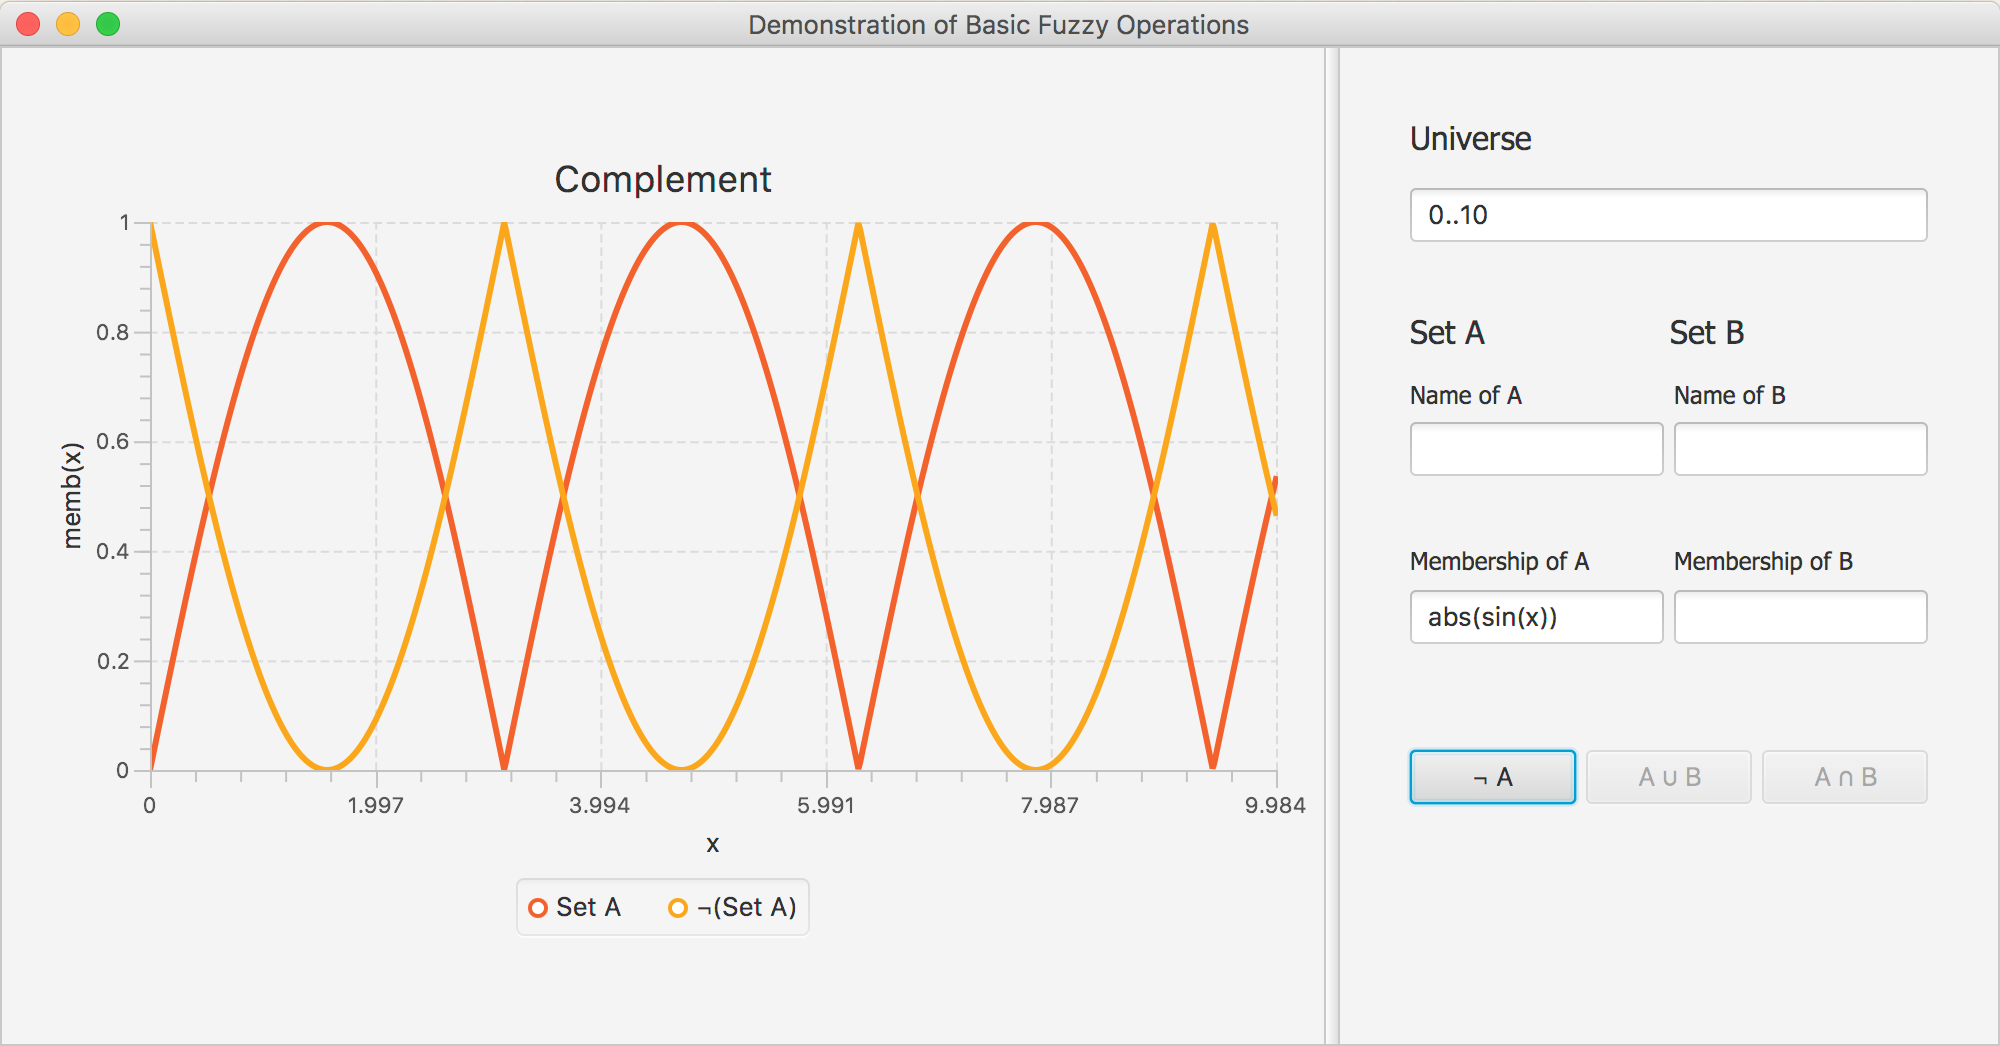
\includegraphics[width=1.0\textwidth]{img/gui}
\caption{The graphical user interface}
\label{fig:gui}
\end{figure}

\paragraph{Error messages}
There are 4 possible error messages in relation to invalid input:
\begin{enumerate}
\item the definition of the universe is not parsable,
\item the membership function is not parsable,
\item the membership function cannot be evaluated,
\item the same name has been given to the fuzzy sets.
\end{enumerate}

A valid universe definition can be either a range, list of several ranges or an enumeration of decimal numbers. In all other cases it invokes an error message which is a hyperlink leading to the Git repository of the project and its \texttt{README} file as seen in Figure \ref{fig:universeDefinitionError}.

The membership function is parsable and evaluable if it is an expression parsable by the \texttt{com.scireum.Parsii} module and it contains exactly one variable, i.e. the \verb|x| in expression \verb|abd(sin(x))|. Otherwise the respective errors would rise up as seen in Figure \ref{fig:membershipParseError} and \ref{fig:membershipEvalError}.

\begin{figure}[!htb]
\minipage{0.32\textwidth}
  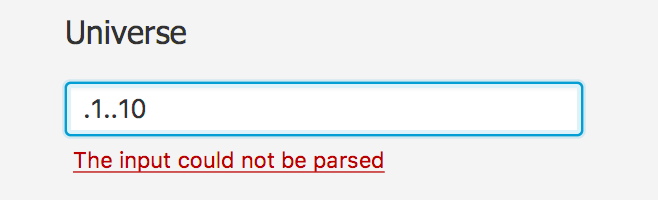
\includegraphics[width=\linewidth]{img/universe-definition-error}
  \caption{Parse error U}\label{fig:universeDefinitionError}
\endminipage\hfill
\minipage{0.32\textwidth}
  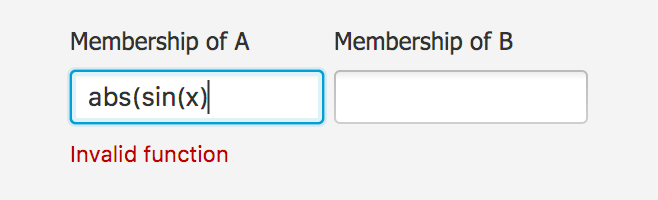
\includegraphics[width=\linewidth]{img/membership-parse-error}
  \caption{Parse error memb()}\label{fig:membershipParseError}
\endminipage\hfill
\minipage{0.32\textwidth}
  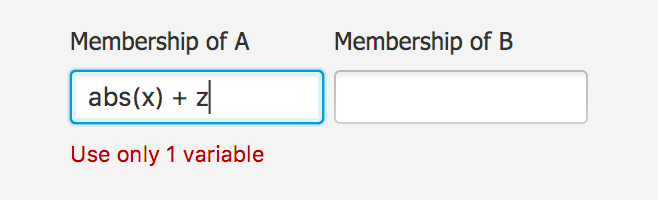
\includegraphics[width=\linewidth]{img/membership-evaluation-error}
  \caption{Eval error memb()}\label{fig:membershipEvalError}
\endminipage
\end{figure}

The fourth error message occurs when both fuzzy sets have been assigned with the same name as it is shown in Figure \ref{fig:setNameError}.

\begin{figure}[!htb]
\minipage{0.45\textwidth}
  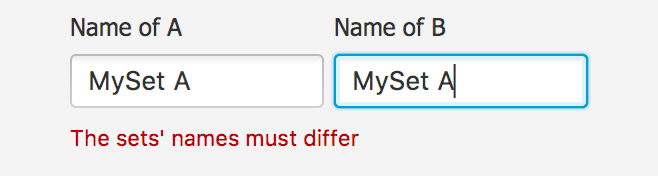
\includegraphics[width=\linewidth]{img/set-name-error}
  \caption{Identical set name error} \label{fig:setNameError}
\endminipage\hfill
\minipage{0.45\textwidth}
  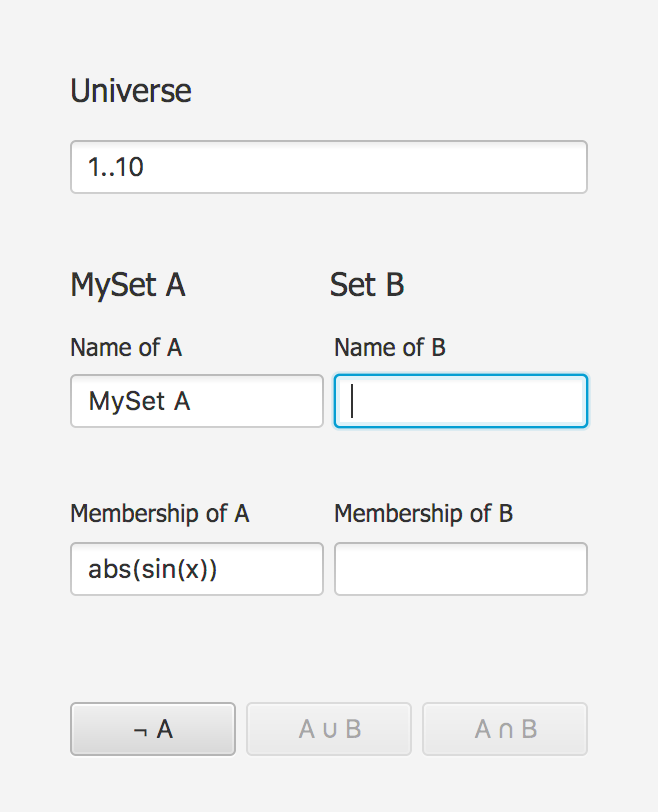
\includegraphics[width=\linewidth]{img/buttons-disabled}
  \caption{Eval error memb()}\label{fig:disabledButtons}
\endminipage
\end{figure}

\paragraph{Action Buttons}
In order to prevent any further errors, the respective action buttons are enabled only in case that all the required fields have been filled out and the input information is valid. The Figure \ref{fig:disabledButtons} shows that the binary operations are disabled when only the first fuzzy set has been set up.

\noindent
\begin{figure}[!h]
\centering
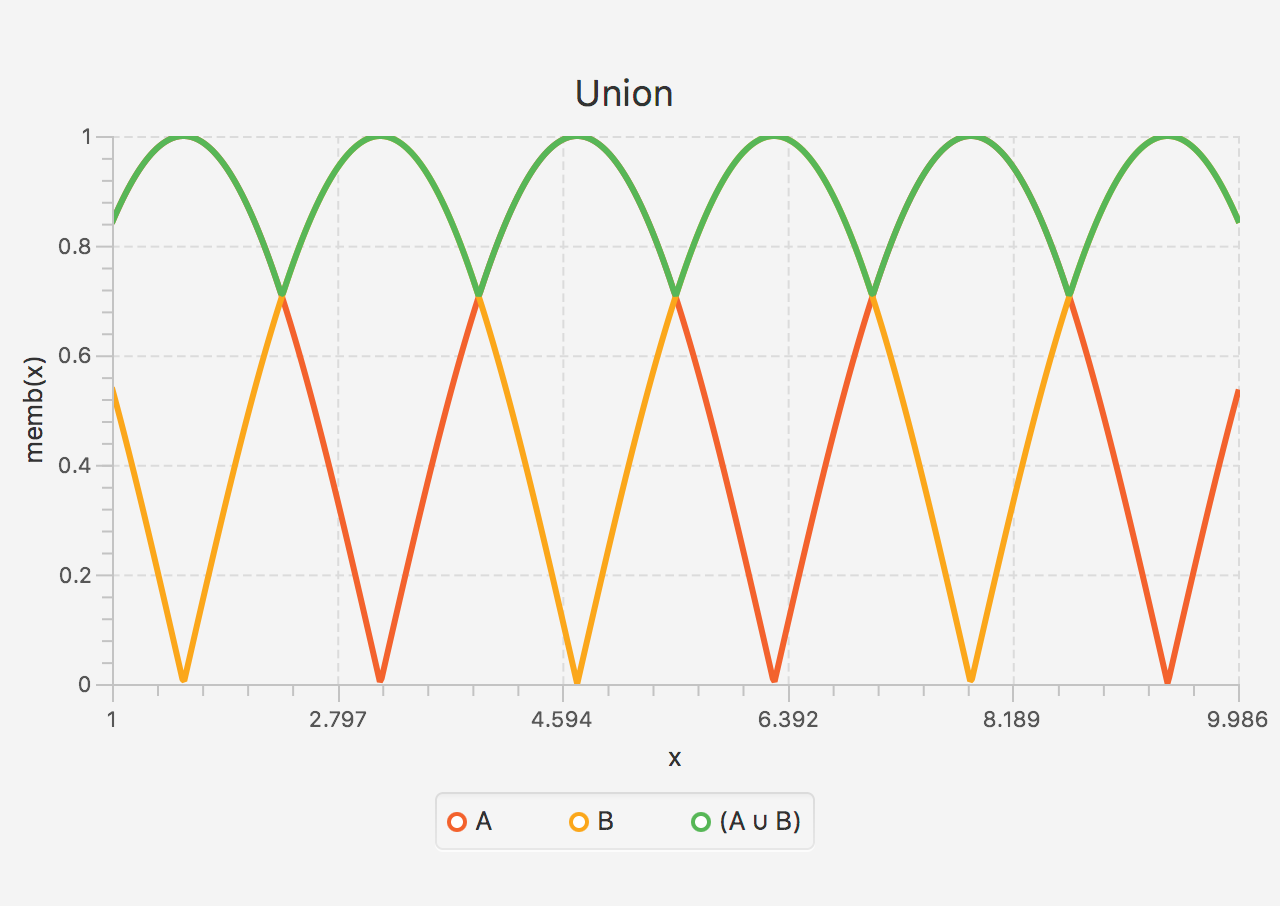
\includegraphics[width=0.7\textwidth]{img/line-chart}
\caption{The line chart}
\label{fig:lineChart}
\end{figure}

\paragraph{Line Chart}
The line chart is the most important element of the UI. It presents the result of the basic operations over the specified fuzzy sets. The following information are always shown to the user, so he is always aware of the currently presented fuzzy operation and its details: \textit{title of the operation}, the \textit{line chart} and the \textit{legend}. An example can be seen in Figures \ref{fig:gui} and \ref{fig:lineChart}.
%=============================================================================
\section{Implementation} \label{implementation}
The desktop application has been implemented in Java 8. It uses the \texttt{com.scireum.Parsii} module to parse and evaluate mathematical expressions. The GUI is implemented using the \texttt{JavaFX 8} library. The tests are written in \texttt{Groovy} using the \texttt{Spock} framework. 

As it has already been mentioned, the application is capable of operating with fuzzy sets defined by a \textit{continuous} universe. In this section we will describe and discuss the implementation of exactly this issue.

\subsection{Discrete vs. continuous}
A digital computer is not able to work with continuous data in their raw form. It uses sampling with an approriate sampling rate to create a set of discrete data it can finally process and operate with. However, the sampling frequency can be set very high, so the produced discrete data may seem for the human eye as continuous. That is exactly the same procedure our desktop application has adopted.

 When a user specifies the universe with a range, e.g. \texttt{0...1}, the application has to decide about the appropriate sampling rate. Too high sampling could be very memory inefficient. On the other hand, too low sampling rate would cause a non-linear member function to loose its \say{curviness}. To find an optimum, the application examines the width of the linechart in pixels. That number is considered as the maximal number of datapoints presented on the chart. Assume the formerly defined universe with the range of \texttt{0...1} and a line chart of a 100 pixels width. It means that the specified interval needs to be discretized into 100 evenly distributed data points across that interval.
 
 The next step is to compute the \textit{precision}. In the above example of a closed range the computation would look as following. Let us assume an unrealistic case of a 5 pixels wide linechart to make the example trivial. The step would be then equal to $\frac{1 - 0}{5 - 1} = 0.25$. If it were a left-closed and right-open range, the computation would be as follows: $\frac{1 - 0}{5} = 0.2$.
 
 \subsection{The algorithm}
 The application operates with only as many datapoints as needed in order to be memory and computation efficient. The following steps describe the workflow that takes place since the start until the end which in our case means that the line chart is populated with data and presented to the user.
 
 \begin{enumerate}
 \item The user enters a \texttt{String} as an input in the universe definition text field.
 	\begin{enumerate}
 	\item The \verb|ApplicationHelper| class checks, whether the input matches an acceptable format.
 	\item If the given input has been evaluated as invalid, the \verb|MainController| sets the error message visible. Otherwise, it does not do anything.
 	\end{enumerate}
\item The user fills out the member function text field.
	\begin{enumerate}
	\item The \verb|MainController| invokes a method chain leading to the \texttt{Parsii} module which parses the member function.
	\item If the given input is not parsable or contains more than 1 variable, an appropriate error message will be set visible.
	\end{enumerate}
\item The user clicks the Complement operation action button.
	\begin{enumerate}
	\item The \verb|MainController| obtains the width of the line chart and sets the \texttt{precision} accordingly.
	\item Then, it creates the universe which is  a \verb|Set| of \verb|FuzzyMember|s generated by the \verb|Range| class.
	\item After the universe is created, the user-specified \verb|FuzzySet| is instantiated.
	\item In the following step, the complement of the instantiated \verb|FuzzySet| is created.
	\item Lastly, the \verb|MainController| populates the line chart with the created fuzzy sets in the exact same order as they have been created. It assures that the data points of the complement fuzzy set will overwrite the data points of the user-specified fuzzy set in the chart.
	\end{enumerate}
 \end{enumerate}
 
 \noindent
\begin{figure}[!h]
\centering
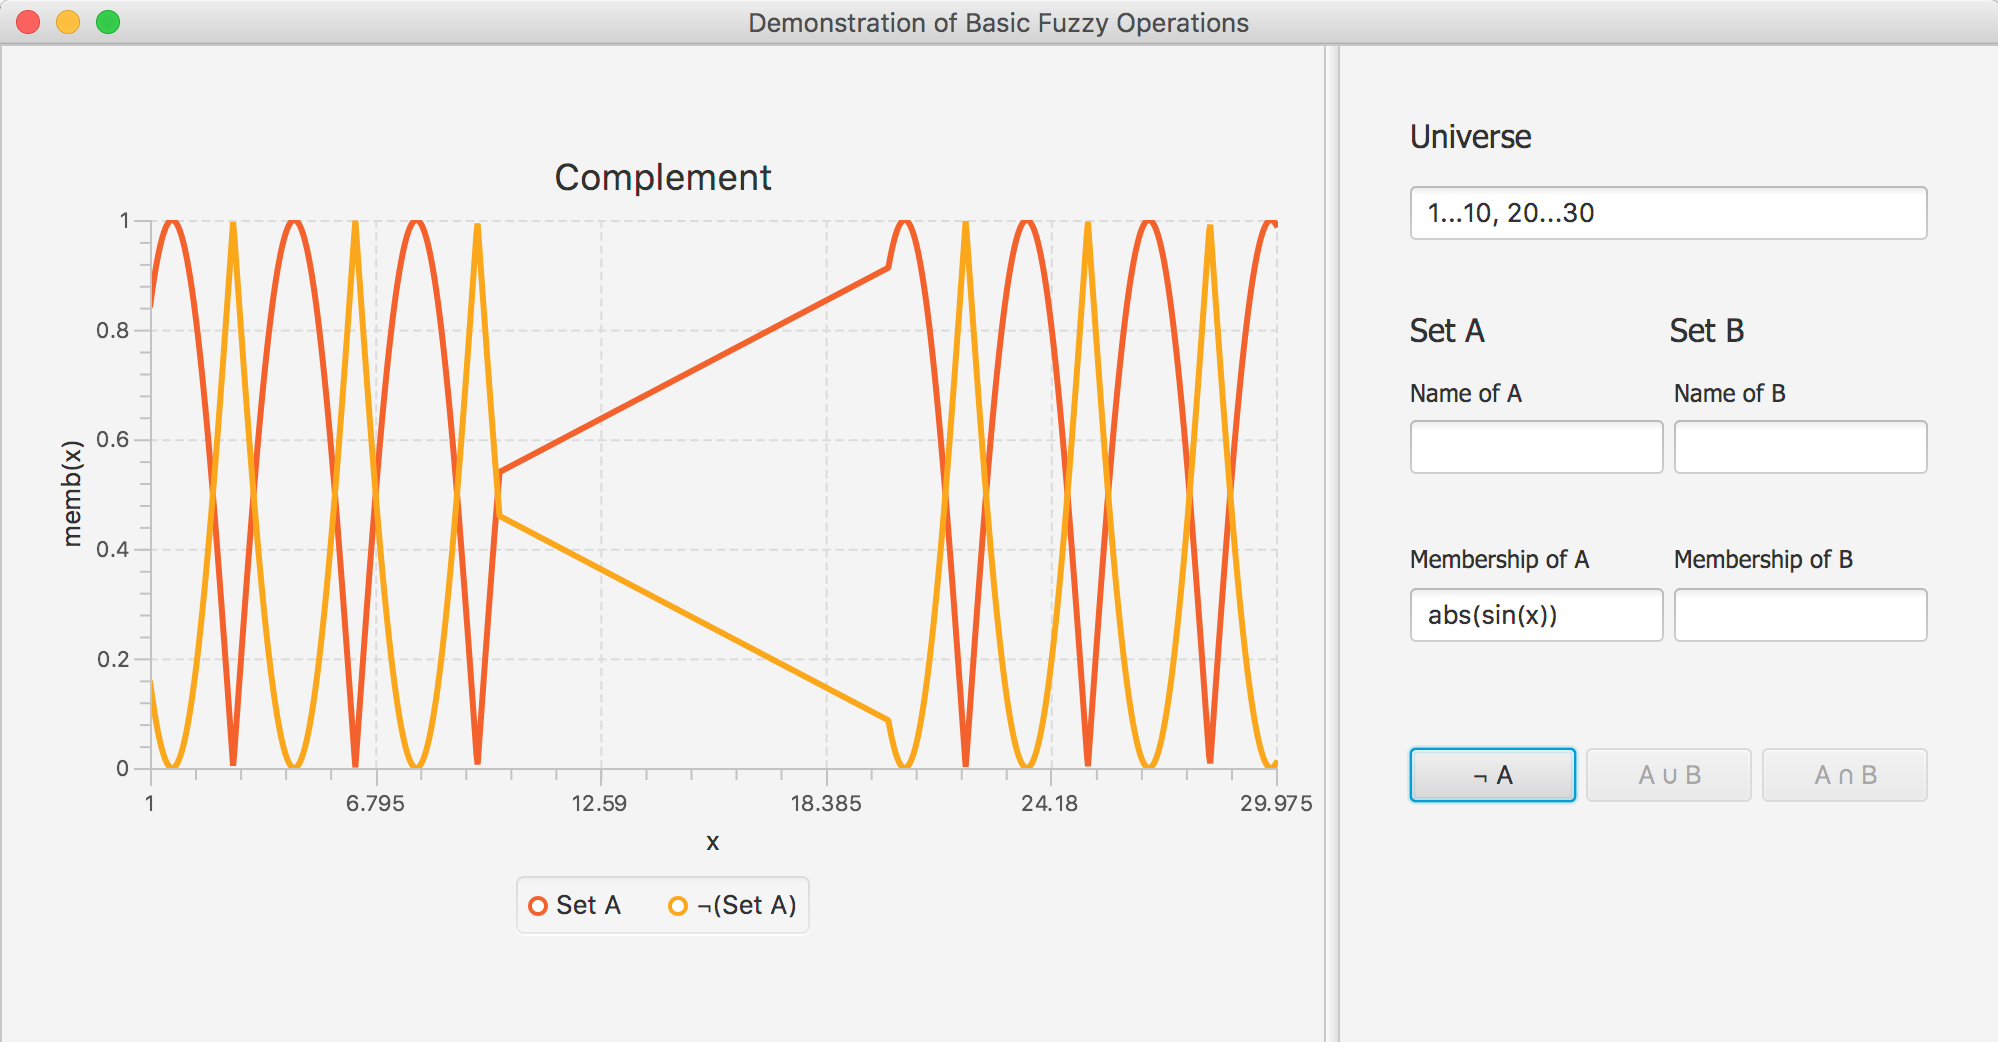
\includegraphics[width=1.0\textwidth]{img/discontinuous-ranges}
\caption{Line chart lacking discontinuity}
\label{fig:discontinuousRanges}
\end{figure}

\subsection{Known issues}
The application is able to present fuzzy sets defined by continuous universes. However, it cannot handle disconinuity. Assume a case when multiple ranges have been specified as the universe by the user, e.g. \verb|1...10, 20...30|. The LineChart of the JavaFX library does not offer any tool to handle such situations. It connects the specified datapoints with a straight line. Having said that, such definitions of the universe may lead to results as seen in Figure \ref{fig:discontinuousRanges}. A possible solution would be to inject another datapoint before the start and after the end of each range with a membership degree of \verb|Double.NaN|. This way the last point of a range and the first point of the following would be connected somewhere outside - in the undefined part of the line chart.

%=============================================================================
\section{Conclusion} \label{conclusion}
This report introduced a desktop application capable of operating with fuzzy sets defined by a continuous univers and a member function as a mathematical expression and demonstrate the 3 basic fuzzy operations over them. We presented the design of the application along with the implementation details and had a more in-depth discussion about challanges met during the development of the project regarding the representation of continuous data sets on a discrete system.

%%%%%%%%%%%%%%%%%%%%%%%%%%%%%%%%%%%%%%%%%%%%%%%%%%%%%%%%%%%%%%%%%%%%%%%%%%%%%%
% seznam citovana literatury: kaada poloaka je definovana paakazem
% \bibitem{xyz}, kde xyz je identifikator citace (v textu pouaij: \cite{xyz})
\newpage
\begin{thebibliography}{1}
\bibitem{fuzzy}
T. Munakata. Fundamentals of the New Artificial Intelligence. Springer Science, 2008
\bibitem{parsii}
Andreas Haufler. scireum/parsii. \url{https://github.com/scireum/parsii}
\bibitem{performanceTest}
Andreas Haufler. How to write one of the fastest expression evaluators in Java? \url{https://www.javacodegeeks.com/2014/01/how-to-write-one-of-the-fastest-expression-evaluators-in-java.html}
\end{thebibliography}

\end{document}
